\chapter{泌尿系统影像解剖}

目前常用的泌尿系影像学检查方法包括KUB+IVP,CT以及MRI,而且尤以后两者在临床应用更为广泛,在本章节中将具体介绍正常MRU及CTU的影像学表现。

\section{检查方法}

MRU以常规成像为基础,通常取冠状面成像。以显示肾门的横断面为定位像设定冠状面层面,以肾门为中心并使成像层面平行于两肾门连线,在冠状面上设定成像视野,视野范围包括双侧肾盂、输尿管、膀胱。

采用3D重T\textsubscript{2} -TSE序列,TR 2000ms,TE
700ms,FOV依病人体型大小而定,多选用360×360,Matix
512×256,层厚2.0mm,无间隔;同时运用脂肪抑制和空间预饱和等相关技术,前者用来抑制周围脂肪高信号,后者用来消除尿路以外液体高信号对尿路图像的影响;图像后处理采用扫描所获得的原始图像进行最大密度投影(maximum
intensity projection,
MIP)重建,其优点是饱和带减少了血管信号强度,观察病变的可疑区而无重叠结构的干扰。

CTU以常规增强成像为基础,常取亦取冠状面成像,成像同样需包括双侧肾盂、输尿管、膀胱。延迟期(排泌期)图像进行薄层重建后,通过后处理软件进行MIP、MPR(多平面重建)或VR(容积再现)等重建技术,观察双侧尿路情况。

\section{重建影像}

以下2幅为MRU图像。
\begin{figure}[!htbp]
 \centering
 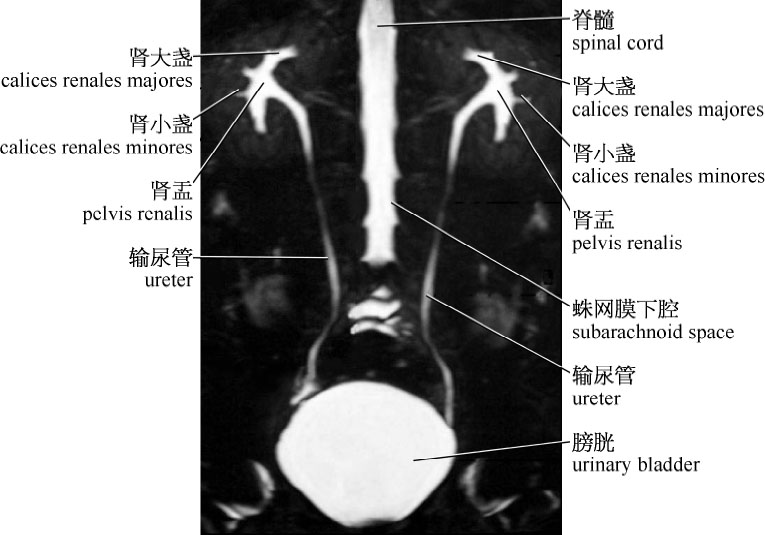
\includegraphics{./images/Image00187.jpg}
  \end{figure} 
 \FloatBarrier

\begin{figure}[!htbp]
 \centering
 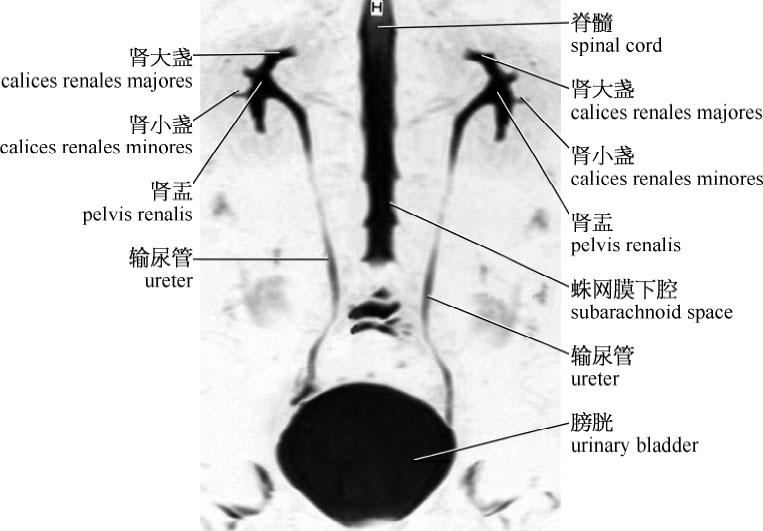
\includegraphics{./images/Image00188.jpg}
  \end{figure} 
 \FloatBarrier



以下2幅为CTU图像。
\begin{figure}[!htbp]
 \centering
 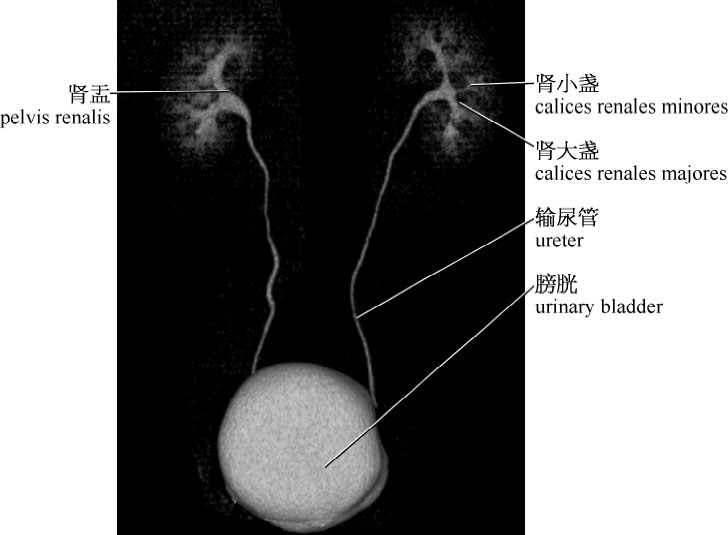
\includegraphics{./images/Image00189.jpg}
  \end{figure} 
 \FloatBarrier

\begin{figure}[!htbp]
 \centering
 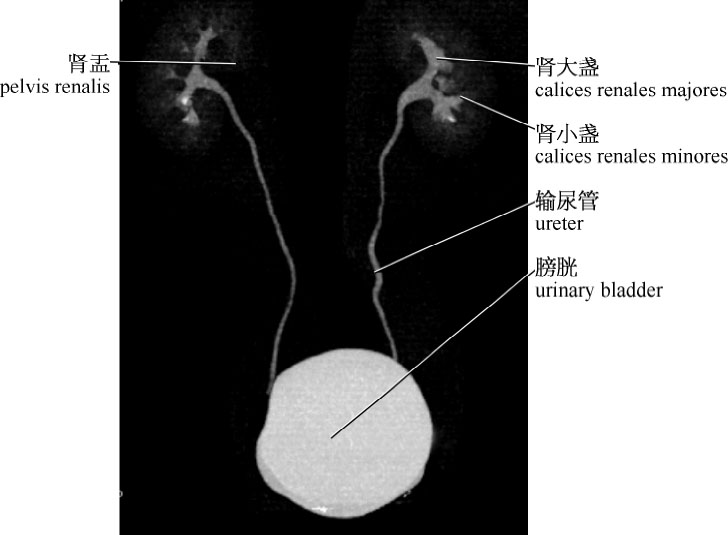
\includegraphics{./images/Image00190.jpg}
  \end{figure} 
 \FloatBarrier

